\documentclass[10pt, conference, compsocconf]{IEEEtran}

\usepackage{amsmath,graphicx,url,float,array}
\usepackage[margin=1in]{geometry}
\raggedbottom
\setlength{\abovecaptionskip}{2pt}
\setlength{\intextsep}{6pt}

\begin{document}

\title{Parallel Alpha-Beta Search for Chess:\\ Preliminary Report}

\author{\IEEEauthorblockN{Bryce Panza, Carter Griffin, Luke Haddad, Samuel Butler, Marco De La Rosa}
\IEEEauthorblockA{School of Informatics, Computing \& Cyber Systems\\
Northern Arizona University, Flagstaff, AZ, U.S.A.}}

\maketitle

\section{Progress Overview}

\subsection*{Framework}

Since this project aims to build out the engine itself rather than a user interface, our progress reflects that goal. We've built out many of the foundational pieces needed to implement future algorithms. These pieces include the following:
\begin{itemize}
\item Board logic and rendering, including the ability to initialize the board, load a given FEN (Forsyth-Edwards Notation)~\cite{edwards1994} board state, and print a simple text-based board to console
\item Game logic, such as piece differentiation, attack logic, check logic, and point values~\cite{shannon1950}
\item Legal move generation, which can generate all legal moves for a given piece and game state
\item Evaluation function which measures the piece relative value for a given gamestate~\cite{shannon1950}
\end{itemize}

\subsection*{Move Generation}

Move generation acts as the fundamental tool for tree traversal in all of our search algorithms.

Each move creates a new copy of the board. Threads read the shared root position concurrently and write only to their own copies. A copy is about 280 bytes, and every version--including the sequential one--performs the same copies. Given how many positions are being searched though this leads to sizable memory usage. Compared to other engines like Stockfish~\cite{stockfish} who use hashes to build transposition tables~\cite{greenblatt1967, zobrist1970}, these hash tables are used to hold previously searched nodes. Each search returns its node count as part of its result.

\subsection*{Board Scoring}

The engine uses material evaluation~\cite{shannon1950} and alpha-beta pruning~\cite{knuth1975}. For material evaluation, each piece has a numerical point value assigned to it. These values are measured in centipawns~\cite{cpwcentipawns}, where 100 centipawns equal 1 pawn or 1 point. As for the other pieces, knights and bishops are worth 300 centipawns or 3 points, rooks are worth 500 centipawns or 5 points, and queens are worth 9 points or 900 centipawns~\cite{shannon1950}. As for evaluating, the engine compares the balance of material from black and white, a positive score indicates an advantage for white and a negative score indicates an advantage for black. The engine omits transposition tables~\cite{greenblatt1967}, quiescence search~\cite{shannon1950}, and the other pruning techniques used in production engines. Stockfish~\cite{stockfish} reaches depth 20 to 30 in the time our engine reaches depth 8. All speedups in this report are relative to our sequential search.

\subsection*{Testing Methodology}

We tested move generation with perft~\cite{cpwperft}, which is used to ensure node count generated on a given position is indeed the correct count. On the starting chess position, a popular benchmark position called Kiwipete~\cite{cpwperft}, and positions 3 through 5. Kiwipete is interesting due to the branching factor it introduces, going from a node count of 48 at depth 1 to 8,031,647,685 at depth 6 while the regular starting position goes from a node count of 20 at depth 1 to 119,060,324~\cite{cpwperft}. These board positions, especially the Kiwipete position, include less common moves like castling, en passant, promotion, and pins. The node counts generated match the published counts on all positions we tested.

\subsection*{Currently Implemented Algorithms}

\subsubsection*{Negamax}

For our baseline sequential algorithm, we are using negamax~\cite{knuth1975}. This algorithm will act as our baseline to compare parallel algorithms against.

As opposed to the standard minimax algorithm~\cite{shannon1950}, negamax evaluates the gamestate for both players using a single maximizing function. It relies on the identity that \mbox{\texttt{max(a, b) = -min(-a, -b)}}~\cite{knuth1975}, and every recursive call negates the returned evaluation (\mbox{\texttt{-negamax(...)}}).

Moves are ordered with captures first. To illustrate the benefits of move ordering, at depth 6, ordering reduced the node count from 664,922 to 297,470 on the start position, from 13,663,041 to 331,111 on Kiwipete, and from 10,585,904 to 237,546 on position 5. Applying MVV-LVA (Most Valuable Victim - Least Valuable Attacker) ordering~\cite{cpwmvvlva} prunes more nodes. We chose captures-first ordering because it is simpler to read. The sequential search is deterministic. It returns the same node count and score on every run, and each parallel result is compared against it.

\subsubsection*{Static Root Split}

Static root split~\cite{marsland1982} is our first and simplest parallelization. This algorithm works by initializing a preset number of threads and shares only the root board and move set. After this point, each thread writes its own arguments, being its node count, score, and best move. Additionally, each node traversal allocates a unique next board state. This removes the need for synchronization. Each thread prunes with its own alpha. The threads together search more nodes than the sequential version. A tradeoff which will be discussed more in the challenges section is that it increases memory overhead significantly, as each node copies the board state.

We reviewed the code on paper for race conditions. The shared data is the root board and the root move list, and the threads only read them. Each thread writes to its own result slot. The main thread reads the slots after \texttt{pthread\_join}~\cite{posix1995} returns. Since each thread writes only to their own slots, the implementation needs no locks, only the barrier of \texttt{pthread\_join}.

As a secondary race-condition check, we ran the code under gcc's ThreadSanitizer~\cite{serebryany2009} for its ability to test for race conditions at runtime. We tested it at 2, 8, and 16 threads, and it reported zero races.

Static root split returns the same evaluation as the sequential search on every benchmark position at every thread count. Limiting the run to a single thread, the static split searches the same number of nodes as our Negamax baseline when given our standardized board test positions.

\section{Challenges}

The proposal planned for 20 physical cores on an Intel i7-14700K. We initially ran the sequential baseline on the host via WSL2, but with the volatility that comes from running tests on a host machine we opted to instead run all parallel experiments run within a Hyper-V Ubuntu VM with 16 virtual CPUs. Running inside a more consistent VM should allow for more accurate speedup times to be measured. As a result however, the thread counts are T in \{1, 2, 4, 8, 12, 16\}, which replaces the range of up to 20 in the proposal. The setup entails the host keeping 12 of its 28 logical CPUs for Windows. Hyper-V reserves 100\% of each of the 16 virtual CPUs for the VM~\cite{msvmprocessor}. We observed the VM baseline to be within 1\% of the earlier WSL baseline. Hyper-V assigns virtual CPUs to physical cores, and above about 8 threads the virtual CPUs run on efficiency cores and hyperthread siblings~\cite{marr2002}.

Each static split thread prunes with its own alpha. At depth 6, Kiwipete searches 331,111 nodes at one thread and 1,122,947 nodes at eight threads, a factor of 3.4. The dynamic split shares alpha between threads to reduce this overhead, so this dynamic approach should solve this.

\section{Remaining Items}

\subsection*{Dynamic Root Split}

The dynamic root split remains to be implemented, measured at each thread count, and reviewed on paper for race conditions. In this algorithm the root moves are placed in a shared FIFO queue. Each idle thread grabs the next move from the queue and searches it. The best score found so far is shared between all threads as $\alpha^{*}$~\cite{marsland1982}. A thread reads $\alpha^{*}$ before it searches a move and updates it when the search returns.

This approach requires more synchronization than static root splitting. The queue and $\alpha^{*}$ are shared by all threads, and each is protected by a mutex~\cite{posix1995}. However, this algorithm should result in greater load balancing, since a thread that finishes a small subtree immediately takes the next move from the queue.

\subsection*{Hybrid Algorithm with Younger Brothers Wait First}

The Young Brothers Wait Concept~\cite{feldmann1989} attempts to reduce the overhead in tree searching by avoiding searching subtrees that would normally be pruned. At each node the younger brothers must wait for the first child, or eldest brother, to be searched sequentially. The younger brothers are searched in parallel, and they are only searched after the eldest brother has returned without a beta cutoff~\cite{feldmann1989}. Parallelism is mostly limited to work the sequential search would also do. A younger brother can still produce a cutoff after its siblings have started, and the abort flag cancels those siblings.

Our hybrid implementation requires the shared work queue from the dynamic root split, the abort flag, a review on paper for race conditions, and a value of \texttt{D\_split} chosen from measurements. \texttt{D\_split} is the minimum remaining depth at which the hybrid pushes a node's younger brothers to the shared queue. Nodes below that depth are searched sequentially by the thread that owns them. In the final report, we will compare speedup, efficiency, and search overhead across all four versions.

\section{Preliminary Results}

Figures 1 through 3 show the static root split results for each benchmark position. Speedup is the sequential time divided by the parallel time. Figure 1 covers response time vs. number of threads in that form.

\begin{table}[H]
\caption{Mean time in seconds, sequential and static root split, depth 8, 5 runs}
\label{tab:times}
\centering
\footnotesize
\begin{tabular}{|c|c|c|c|c|}
\hline
T & Start & Kiwipete & Pos. 4 & Pos. 5 \\
\hline
Seq & 2.617 & 14.775 & 3.505 & 7.541 \\
\hline
1 & 2.617 & 14.753 & 3.448 & 7.569 \\
2 & 1.411 & 8.574 & 2.151 & 4.431 \\
4 & 0.914 & 5.982 & 1.871 & 3.178 \\
8 & 0.614 & 4.167 & 1.398 & 2.081 \\
12 & 0.675 & 4.264 & 1.414 & 2.002 \\
16 & 0.558 & 3.637 & 1.429 & 1.996 \\
\hline
\end{tabular}

\end{table}

Search overhead is the total nodes searched by all threads divided by the nodes searched by the sequential version~\cite{marsland1982}. In the sequential search the result of each move shrinks the alpha-beta window for every move after it. In the static root split, each thread only has the results of its own moves. The threads end up searching nodes that the sequential search prunes. A search overhead of 2 means the threads searched twice as many nodes as the sequential version. We include it as a third plot.

Figures 1 and 2 show the speedup and efficiency of the static root split on each of the four positions.

\begin{figure}[H]
\centering
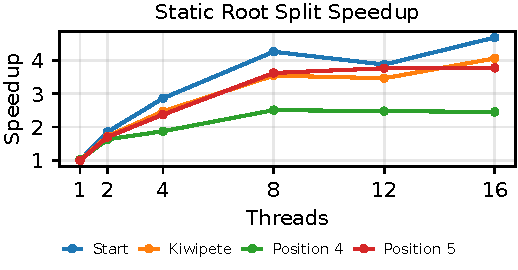
\includegraphics[width=0.92\columnwidth]{figures/static_speedup.pdf}
\caption{Static root split speedup vs. threads, depth 8, VM with 16 vCPUs}
\label{fig:speedup}
\end{figure}

\begin{figure}[H]
\centering
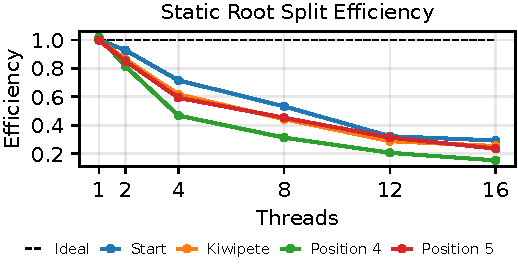
\includegraphics[width=0.92\columnwidth]{figures/static_efficiency.pdf}
\caption{Static root split efficiency vs. threads}
\label{fig:efficiency}
\end{figure}

\begin{figure}[H]
\centering
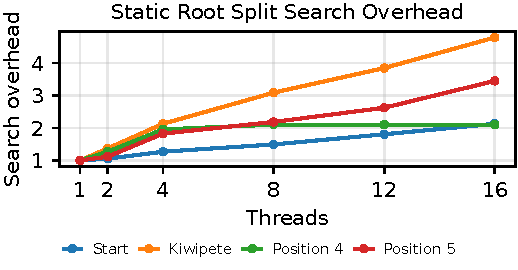
\includegraphics[width=0.92\columnwidth]{figures/static_overhead.pdf}
\caption{Static root split search overhead vs. threads}
\label{fig:overhead}
\end{figure}

We removed perft position 3 from the benchmark set. It finishes in about 0.1 seconds at depth 8 so it is too short to see meaningful performance differences at the same depth as other tests.

Position 4 starts with white in check and has only 6 legal moves at the root. Static root split gives each root move to one thread. At most 6 threads have work and the rest get nothing. Speedup levels off around 2.5 from 8 threads on and the node count stays at 28,535,788. Efficiency is 2.5 / T past that point. It falls from 0.31 at 8 threads to 0.15 at 16.

Efficiency falls on every position as thread count increases. At 8 threads the static split keeps 0.31 to 0.53 efficiency. Going from 8 to 16 threads adds 0.16 to 0.51 speedup on start, Kiwipete and position 5 and nothing on position 4. Preliminarily, it appears that 8 threads is the best tradeoff for the static split.

\section{Checklist}\label{sec:checklist}

It is worth noting that we completed the November 13 and November 16 milestones on the same date, November 18th, which is a deviation from the original proposal.

\begin{table}[H]
\label{tab:checklist}
\centering
\footnotesize
\renewcommand{\arraystretch}{1.0}
\setlength{\tabcolsep}{3pt}
\begin{tabular}{|>{\centering\arraybackslash}m{0.62in}|m{1.85in}|>{\centering\arraybackslash}m{0.38in}|}
\hline
\textbf{Date} & \centering\arraybackslash\textbf{Milestone} & \textbf{Status} \\
\hline
November 13 & We intend to have all sequential searches running on real chess positions. All parallel versions will be compared against these. & DONE \\
\hline
November 16 & We plan to have the static root split implemented and measured at each thread count. Its code will also be reviewed on paper for race conditions. These results will be included in the preliminary report. & DONE \\
\hline
November 23 & We intend to have the dynamic root split implemented and measured at each thread count. Its code will also be reviewed on paper for race conditions. & TODO \\
\hline
December 3 & We plan to have the hybrid implemented on the shared work queue. This includes the abort flag for cancelling sibling tasks after a beta cutoff, which we expect to be the hardest part of the implementation (and most interesting). Its code will also be reviewed on paper for race conditions, and $D_{split}$ will be chosen from its measurements. & TODO \\
\hline
December 10 & We will submit the final report comparing the speedup, efficiency, and search overhead of all four versions. & TODO \\
\hline
\end{tabular}
\end{table}

\bibliographystyle{IEEEtran}
\bibliography{biblio}

\end{document}
